%% ============================================================
%%  RutAI --- Manuscript for Pervasive and Mobile Computing
%%  Elsevier CAS Single-Column class (cas-sc.cls)
%%  Bundle: els-cas-templates (v2.4)
%% ============================================================

\documentclass[a4paper,fleqn]{cas-sc}

% Author-year citations with long first citation, standard for PMC.
\usepackage[authoryear,longnamesfirst]{natbib}

\usepackage{amsmath,amssymb,amsthm}
\usepackage{graphicx}
\usepackage{booktabs}
\usepackage{multirow}
\usepackage{url}
\usepackage{hyperref}
\usepackage[utf8]{inputenc}
\usepackage[T1]{fontenc}
\usepackage{xcolor}
\usepackage{algorithm}
\usepackage{algpseudocode}
\usepackage{tikz}
\usetikzlibrary{arrows.meta, positioning, shapes.geometric, fit, calc}

\def\tsc#1{\csdef{#1}{\textsc{\lowercase{#1}}\xspace}}
\tsc{RUTAI}
\tsc{GPS}
\tsc{IOT}
\tsc{LBS}
\tsc{POI}
\tsc{UCB}
\tsc{MAB}
\tsc{TAM}
\tsc{CBSE}
\tsc{MVVM}

\begin{document}
	\let\WriteBookmarks\relax
	\def\floatpagepagefraction{1}
	\def\textpagefraction{.001}
	
	% ---------- Running heads ------------------------------------------
	\shorttitle{RutAI: AI-driven geolocated alarms for urban routing}
	\shortauthors{A.~Reyes et~al.}
	
	% ---------- Title --------------------------------------------------
	\title[mode=title]{RutAI: A Component-Based Mobile Framework Integrating Bandit-Learned Route Alternation, Geolocated Alarms and Collaborative Monitoring for Safer Urban Mobility}
	
	\tnotemark[1]
	
	\tnotetext[1]{This research was carried out at the Faculty of Computer Sciences, Universidad T\'ecnica Estatal de Quevedo, in collaboration with the Department of Software Engineering of the Universidad de Granada.}
	
	% ---------- Authors ------------------------------------------------
	\author[1]{Aar\'on Reyes}[orcid=0000-0000-0000-0000]
	\ead{aaron.reyes@uteq.edu.ec}
	\credit{Conceptualization, Software, Methodology, Validation, Writing --- original draft}
	
	\author[1]{Gleiston Guerrero-Ulloa}[orcid=0000-0000-0000-0000]
	\cormark[1]
	\ead{gguerrero@uteq.edu.ec}
	\credit{Supervision, Conceptualization, Methodology, Writing --- review \& editing}
	
	\author[2]{Miguel~J.~Hornos}[orcid=0000-0000-0000-0000]
	\ead{mhornos@ugr.es}
	\credit{Formal analysis, Writing --- review \& editing, Validation}
	
	\author[2]{Carlos Rodr\'iguez-Dom\'inguez}[orcid=0000-0000-0000-0000]
	\ead{carlosrodriguez@ugr.es}
	\credit{Methodology, Writing --- review \& editing, Validation}
	
	\author[1]{Efra\'in D\'iaz-Mac\'ias}[orcid=0000-0000-0000-0000]
	\ead{ediazm@uteq.edu.ec}
	\credit{Investigation, Resources, Writing --- review \& editing}
	
	\affiliation[1]{organization={Faculty of Computer Sciences, Universidad T\'ecnica Estatal de Quevedo},
		addressline={Av.~Quito Km.~1 V\'ia a Santo Domingo},
		city={Quevedo},
		postcode={120301},
		state={Los R\'ios},
		country={Ecuador}}
	
	\affiliation[2]{organization={Department of Software Engineering, Universidad de Granada},
		addressline={C.~Periodista Daniel Saucedo Aranda s/n},
		city={Granada},
		postcode={18014},
		country={Spain}}
	
	\cortext[1]{Corresponding author.}
	
	% ---------- Structured abstract (Elsevier style) -------------------
	\begin{abstract}
		\textbf{Background:} Urban commuters in Latin American cities frequently follow repetitive and predictable routes, forget context-bound errands during their trips, and lack integrated tools to coordinate their movements with trusted peers. Most existing mobile solutions tackle route recommendation, location-based reminders, and collaborative tracking in isolation, which limits their joint contribution to perceived safety and daily efficiency.
		\textbf{Objective:} This paper introduces \RUTAI{}, a component-based mobile framework that unifies (i) bandit-learned alternative routing, (ii) geofence- and time-triggered reminders, and (iii) privacy-controlled collaborative monitoring into a single pervasive system for urban mobility.
		\textbf{Methods:} \RUTAI{} is designed following Component-Based Software Engineering (\CBSE{}) across six phases: requirements specification, component analysis, evaluation and selection, assembly and integration, verification and validation, and deployment. The Android client is built with Kotlin, Jetpack Compose, and a Model-View-ViewModel (\MVVM{}) architecture; the backend uses Python, FastAPI, PostgreSQL, and Redis, with WebSocket-based real-time communication. Route personalization relies on a Multi-Armed Bandit algorithm with an Upper Confidence Bound (\UCB{}) policy that balances exploration and exploitation of per-destination route types. Acceptance was evaluated with 25 participants using an extended Technology Acceptance Model (\TAM{}) that incorporates Perceived Security as a fifth construct.
		\textbf{Results:} All five \TAM{} constructs exceeded the 3.5 acceptance threshold on a 5-point Likert scale: Perceived Usefulness $\mu{=}4.14$, Perceived Ease of Use $\mu{=}4.18$, Attitude Toward Use $\mu{=}4.13$, Intention to Use $\mu{=}4.12$, and Perceived Security $\mu{=}4.29$. The instrument's global Cronbach's $\alpha=0.986$, indicating excellent internal consistency. Pearson correlations between constructs were uniformly high ($r>0.94$), and Perceived Security showed the most compact response distribution.
		\textbf{Conclusions:} \RUTAI{} demonstrates that integrating bandit-based route personalization, geofencing, and real-time collaborative tracking in a single component-based architecture is technically feasible and well received by first-time users. The framework advances the state of the art in pervasive and mobile urban-mobility systems by providing an end-to-end, reproducible design aligned with Sustainable Development Goal 11 on safer and more inclusive cities.
	\end{abstract}
	
	% ---------- Highlights ---------------------------------------------
	\begin{highlights}
		\item \RUTAI{} unifies bandit-learned routing, geofenced reminders, and collaborative tracking.
		\item A UCB multi-armed bandit personalises route-type choice per destination.
		\item Component-based Android + FastAPI design supports offline use and WebSocket real-time.
		\item Five TAM constructs exceed 3.5; global Cronbach's $\alpha=0.986$.
		\item Perceived Security scores 4.29, the highest of the five evaluated constructs.
	\end{highlights}
	
	% ---------- Keywords -----------------------------------------------
	\begin{keywords}
		Pervasive mobile computing \sep Geolocated reminders \sep
		Multi-armed bandit \sep Context-aware routing \sep
		Collaborative location sharing \sep Technology Acceptance Model
	\end{keywords}
	
	\maketitle
	
	% ==================================================================
	\section{Introduction}\label{sec:intro}
	% ==================================================================
	
	Cities are the stage on which most of human activity unfolds. According to the United Nations Department of Economic and Social Affairs (UN-DESA), the 2025 Revision of the World Urbanization Prospects estimates that $57\%$ of the world's population lived in urban areas in 2025 and projects that this share will reach $68\%$ by 2050, with Latin America and the Caribbean already above $82\%$ urbanisation \citep{undesa2025wup}. At the individual scale, human trajectories are remarkably regular: the seminal entropy study of \citet{song2010predictability} showed a theoretical predictability ceiling of $93\%$ for mobile-phone-derived traces, a finding repeatedly confirmed by subsequent work on large-scale mobility mining \citep{cagney2025urban,liu2022route}. This combination of dense urbanisation and predictable daily travel patterns delimits a research space where pervasive and mobile computing can deliver large gains in efficiency, wellbeing, and safety.
	
	That same regularity, however, turns into a liability when cities carry high crime pressure. The World Bank's 2025 regional outlook documents that Latin America and the Caribbean concentrate about one-third of the world's homicides despite hosting less than $10\%$ of its population \citep{maloney2025worldbank}, a figure corroborated by the International Monetary Fund's macroeconomic analysis of violent crime in the region \citep{bisca2024violent} and by the UN Office on Drugs and Crime (UNODC) 2023 Global Study on Homicide for Latin America and the Caribbean \citep{unodc2023gshlac}. In high-pressure contexts, repeating the same commuting route day after day makes a person easy to profile and exposes her to predictable-trajectory attacks; in high-density megacities with complex public-transit systems, the same routine limits the ability to adapt to incidents in real time. These pressures motivate a class of pervasive mobile services that (i)~diversify routes without sacrificing convenience, (ii)~externalise memory so that errands tied to specific places or moments are not forgotten, and (iii)~enable trusted peers to coordinate in real time.
	
	\subsection{Motivation and research problem}\label{sec:motivation}
	
	The problem is shared across very different urban contexts. In Mexico City, the National Survey of Urban Public Safety (ENSU) reported that $58.6\%$ of adults felt unsafe in their city in mid-2024 \citep{unodc2023gshlac}, and the perception of insecurity was shown to reshape daily mobility decisions such as time of travel and route choice \citep{maloney2025worldbank}. In Bogot\'a, the city government's 2024 security reports place theft rates at $22.9$ incidents per thousand inhabitants, well above European capitals \citep{bisca2024violent}. In S\~ao Paulo, perception surveys place the city among the lowest in trust in public safety in the hemisphere despite declining homicide rates \citep{unodc2023gshlac}. In smaller Ecuadorian cities such as Quevedo, local survey evidence reports that $96.8\%$ of university students express fear of victimisation in their daily routines \citep{tapia2024inseguridad}. These four cities differ in size and context, yet they converge on the same need: users perceive that their commuting routine is too predictable, that they forget context-bound errands along the way, and that informal coordination channels are insufficient to convey a real-time sense of whereabouts to family and peers.
	
	Three independent bodies of evidence reinforce the motivation for an integrated response. First, individual trajectories concentrate most of their mass on a small set of preferred locations \citep{cagney2025urban,liu2022route,song2010predictability}, so the exploration of alternative routes must be actively promoted by the system. Second, cognitive-science evidence shows that intentions tied to contextual cues are systematically under-fulfilled unless they are externalised as location-aware or time-aware reminders \citep{rummel2023prospective,ball2025offloading}. Third, commuters already improvise real-time coordination using calls and text messages, but this ad-hoc channel is neither continuous nor reliable; dedicated, privacy-aware real-time substrates have been repeatedly proposed as a better substrate \citep{li2017locsharing,mckenzie2022privyto,shokri2014mobicrowd}. None of these three strands, in isolation, addresses the whole phenomenon.
	
	The overarching research question is therefore: \emph{how can route diversification, context-aware reminders, and collaborative location sharing be combined in a single component-based mobile framework that is accepted by end users and that contributes to perceived safety during urban travel?} This question is explicitly framed at the intersection of pervasive computing, mobile human--computer interaction, and urban-mobility informatics, which is the target scope of \emph{Pervasive and Mobile Computing}.
	
	\subsection{Contributions and paper organisation}\label{sec:contrib}
	
	In answering this question, the paper makes five contributions, framed as responses to gaps identified in Section~\ref{sec:related}:
	
	\begin{itemize}
		\item A unified, component-based Android $+$ FastAPI architecture that composes route alternation, geofenced reminders, and collaborative monitoring under the same \MVVM{} and Repository patterns, enabling independent evolution of each module.
		\item A route-personalization mechanism based on the Multi-Armed Bandit (\MAB{}) algorithm with an \UCB{} policy that treats each destination as an independent bandit instance and balances exploration of alternative route types against exploitation of previously preferred ones.
		\item A geofencing subsystem that supports compound spatial conditions and time-constrained triggers, aligned with recent methodological requirements for behavioural research on geofencing \citep{shevchenko2024geofencing}.
		\item A WebSocket-based collaborative monitoring module with privacy-aware group membership and message read/write receipts, addressing the reported mismatch between existing privacy-first platforms and the need for real-time coordination \citep{li2017locsharing,mckenzie2022privyto}.
		\item An empirical acceptance study with 25 participants using an extended Technology Acceptance Model (\TAM{}) instrument, in which Perceived Security is treated as a first-class construct, as the Latin American urban context arguably demands.
	\end{itemize}
	
	The remainder of the paper is organised as follows. Section~\ref{sec:related} groups the related work by common themes and derives the research gap. Section~\ref{sec:method} describes the materials and methods, including the Component-Based Software Engineering (\CBSE{}) development process and the statistical procedures. Section~\ref{sec:results} reports the implementation outcomes and the acceptance results. Section~\ref{sec:discussion} discusses the findings against the literature. Section~\ref{sec:conclusion} concludes and outlines future work.
	
	% ==================================================================
	\section{Related Work}\label{sec:related}
	% ==================================================================
	
	The related literature spans three complementary streams: route personalization, location-based reminders, and collaborative location sharing. We review each stream in a way that lets us compare the reviewed works against each other rather than listing them, and close the section by consolidating the shared deficiencies that motivate \RUTAI{}.
	
	\subsection{Route personalization and smart-mobility recommendation}\label{sec:rw-routes}
	
	The first stream applies machine-learning and online-learning techniques to route and multimodal transport recommendation. \citet{yuan2022mlits} survey machine-learning techniques for next-generation intelligent transportation systems and highlight scalability and data-volume constraints as the main bottlenecks for practical deployment; this survey is particularly useful because it positions the subsequent, more specific contributions within a common taxonomy. Within that taxonomy, the online-learning method of \citet{guo2021online} can be read as a representative of the \emph{short-horizon reactive} family: it couples traffic forecasting with route adjustment and reports reductions in travel time on urban traffic traces. \citet{liu2022multimodal} are positioned, by contrast, in the \emph{long-horizon personalised} family: their multitask deep-learning framework for multimodal transport recommendation is highly expressive but presupposes large, multi-source datasets (transport APIs, POI layers, user logs), which effectively raises the bar for deployment. Compared against \citet{campigotto2017favour}'s earlier FAVOUR recommender, which was already situation- and preference-aware, \citet{liu2022multimodal} and \citet{guo2021online} trade expressiveness against reproducibility in contexts with limited data.
	
	A more recent branch applies deep reinforcement learning to urban traffic and swarm-scale routing. \citet{zhang2025drlnavigation} demonstrate that hierarchical DRL can coordinate vehicle swarms and optimise traffic, while \citet{kuhnle2021rl} show analogous benefits in adaptive production control, thus supporting the generality of the approach. These works are attractive for their performance ceilings but, relative to \citet{campigotto2017favour} and \citet{guo2021online}, they further amplify the computational and data requirements, and they inherit the well-known interpretability and cold-start issues of DRL. This is where the \MAB{} literature becomes relevant as a simpler and more transparent alternative. \citet{bouneffouf2020mabsurvey} offer a comprehensive survey that places contextual and classical bandits under a common umbrella; within that umbrella, \citet{zeng2016mab} target online context-aware recommendation with time-varying arms, and \citet{shi2021fedmab} extend the formulation to a federated setting. Compared directly, \citet{shi2021fedmab} keep the learning process per-user while aggregating aggregate statistics, which is precisely the privacy property that route recommenders for urban mobility ideally want but rarely achieve.
	
	Taken together, three common deficiencies recur across this stream. First, most proposals rely on large training corpora that are usually unavailable in medium-sized Latin American cities. Second, they optimise for travel time or cost and do not treat route \emph{diversification} (a safety-oriented objective) as a first-class target, despite the empirical evidence that mobility patterns are highly predictable \citep{song2010predictability,cagney2025urban,liu2022route}. Third, they are treated in isolation from reminders or collaborative tracking, which limits their overall user-level impact. These deficiencies are explicitly consolidated in Section~\ref{sec:rw-summary}.
	
	\subsection{Location-based reminders and geofencing}\label{sec:rw-reminders}
	
	The second stream targets location-triggered reminders. Early work by \citet{lin2014lbr} proposed a location-based personal task reminder for Android using IEEE~802.11 WLAN infrastructure for both indoor and outdoor triggers. This proposal defined the functional skeleton of subsequent location-based reminders: a point, a radius, and an enter/exit trigger. What \citet{garzon2014geofencing} contribute on top of this skeleton is expressivity: they formalise compound geofencing scenarios, where the notification depends on the sequential crossing of multiple virtual fences. This shift from single- to compound-fence logic is significant because it moves the reminder space from context-free alerts to context-rich ones, without which reminders tied to errands during a trip cannot be expressed precisely. \citet{wang2015beyond} complement this contribution by arguing, on CHI, that even compound fences are a restricted language for specifying location in reminders and proposing a more expressive space that accommodates semantic locations and trajectories.
	
	More recently, \citet{shevchenko2024geofencing} consolidated the methodological discussion with a full behavioural-research framework for geofencing that specifically addresses two issues that prior work downplayed: (i)~the privacy cost of continuous background tracking and (ii)~battery drain due to unrestricted GPS polling. The contrast with \citet{lin2014lbr} and \citet{garzon2014geofencing} is instructive: while the earlier works focused on what the system can \emph{detect}, \citet{shevchenko2024geofencing} focus on what the system can detect \emph{at an acceptable cost} to the user's device and privacy. In parallel, cognitive-science evidence provides the psychological justification for geofenced reminders. \citet{rummel2023prospective} show, in a natural-environment study, that prospective memory tasks are forgotten at significantly higher rates than retrospective ones, while \citet{ball2025offloading} demonstrate that participants offload prospective memory onto external reminders primarily to avoid cognitive costs rather than to boost accuracy, which matters for user-interface design.
	
	From a comparison perspective, three deficiencies consistently emerge across this stream. First, most reminder systems do not expose their triggers to other modules of the application, which means that a reminder cannot change a route choice, and a route choice cannot re-prioritise reminders. Second, time-based and location-based triggers are typically treated as separate modalities even when the user mental model couples them (``when I pass the pharmacy on my way home''). Third, user studies seldom consider the sense of security that a well-timed reminder generates during urban travel, focusing instead on productivity metrics. \RUTAI{} responds to all three gaps.
	
	\subsection{Collaborative monitoring and privacy-preserving location sharing}\label{sec:rw-collab}
	
	The third stream addresses how users can share their location with trusted peers. \citet{li2017locsharing} present a multi-server architecture for location sharing in mobile online social networks, designed so that no single server holds enough information to reconstruct the user's trajectory. \citet{mckenzie2022privyto} propose PrivyTo, a privacy-preserving location-sharing platform that represents a more recent and lightweight alternative in the same design space. Compared directly, \citet{li2017locsharing} pay a heavier engineering price (multi-server coordination) for stronger guarantees, whereas \citet{mckenzie2022privyto} trade some guarantees for deployability. Neither of the two prioritises real-time group messaging with delivery and read receipts, which is precisely the missing dimension when the system is used in an insecure urban context where peers want to \emph{know now} where the user is.
	
	A more radical design is \citet{shokri2014mobicrowd}'s MobiCrowd, which shifts location-privacy protection to the user crowd itself: mobile devices share context through a cache-like mechanism so that the LBS is queried as little as possible. Compared against \citet{li2017locsharing} and \citet{mckenzie2022privyto}, MobiCrowd is more distributed, but it is also harder to reason about in small or sparse cities where the crowd is thin. A complementary line of work, represented by the crime-safety map of \citet{kim2025crimesafetymap}, shows that the map-centric paradigm can be extended with geofenced alerts around risky areas, tightening the link between location sharing and perceived safety. Relative to the privacy-first designs, \citet{kim2025crimesafetymap} accept richer data (crime records by area) and obtain richer alerts in return, which is an opposite trade-off along the privacy--utility axis.
	
	When the three streams are overlaid, three concrete deficiencies emerge in the collaborative-monitoring space. First, privacy-first designs rarely offer real-time, group-level communication with read receipts. Second, location sharing is not coordinated with the user's route choices, which means that a user who deviates from a predicted route cannot be flagged proactively. Third, the cognitive and emotional role of sharing locations with trusted peers ---as opposed to the engineering problem of leakage--- is underspecified in the literature. The \RUTAI{} design takes an explicit stance on each of these three points.
	
	\subsection{Summary of deficiencies and positioning of \RUTAI{}}\label{sec:rw-summary}
	
	Cross-cutting the three streams reviewed in Sections~\ref{sec:rw-routes}--\ref{sec:rw-collab}, we consolidate the common deficiencies into five explicit gaps. The citations supporting each gap are those already introduced in the preceding subsections; no new literature is added here, so that the summary remains strictly a synthesis of the reviewed body of work.
	
	\begin{enumerate}
		\item \emph{Integration gap}: no prior system combines route personalization, geofenced reminders, and real-time collaborative monitoring under a single coherent architecture. ML-based routing \citep{yuan2022mlits,guo2021online,liu2022multimodal,campigotto2017favour}, reminder systems \citep{lin2014lbr,garzon2014geofencing,wang2015beyond,shevchenko2024geofencing} and collaborative platforms \citep{li2017locsharing,mckenzie2022privyto,shokri2014mobicrowd,kim2025crimesafetymap} are consistently studied and built as independent silos, and this fragmentation is explicitly acknowledged in the smart-mobility surveys \citep{paiva2021smartmobility,kung2023lbs}.
		\item \emph{Data-scarcity gap}: most ML-based mobility solutions assume large training corpora that are unavailable in medium-sized Latin American cities \citep{yuan2022mlits,liu2022multimodal,zhang2025drlnavigation}. Multi-armed bandit formulations are a known remedy under sequential-decision uncertainty \citep{bouneffouf2020mabsurvey,zeng2016mab,shi2021fedmab}, but they have not been exploited as the learning engine of an end-to-end mobile framework.
		\item \emph{Safety-oriented routing gap}: traditional route recommenders optimise for time or cost \citep{campigotto2017favour,guo2021online,liu2022multimodal,zhang2025drlnavigation}, while route \emph{diversification} to reduce predictability is rarely formulated as a first-class objective, even though empirical evidence shows that commuting patterns are highly repetitive \citep{song2010predictability,cagney2025urban,liu2022route} and that this predictability is a liability in insecure urban settings \citep{tapia2024inseguridad,maloney2025worldbank}.
		\item \emph{Real-time privacy gap}: privacy-preserving location-sharing platforms \citep{li2017locsharing,mckenzie2022privyto,shokri2014mobicrowd} prioritise anonymity and minimal disclosure but typically sacrifice real-time group communication with delivery and read receipts, leaving the design space between privacy and coordination underexplored.
		\item \emph{Evaluation gap}: acceptance studies for this family of systems seldom treat \emph{Perceived Security} as a separate, first-class construct alongside the classical \TAM{} dimensions \citep{davis1989tam}, despite its salience in Latin American urban contexts \citep{tapia2024inseguridad,maloney2025worldbank} and the need for principled Likert-scale interpretation in this kind of evaluation \citep{lindner2024likert}.
	\end{enumerate}
	
	Against this backdrop, \RUTAI{} proposes a single, reproducible, component-based framework that (1)~couples a \UCB{} bandit \citep{bouneffouf2020mabsurvey,zeng2016mab} with route-diversification as a safety goal, going beyond the time/cost objectives of \citet{campigotto2017favour} and \citet{guo2021online}; (2)~unifies time- and location-based triggers in a reminder module that is aware of both the route and the group context, operationalising the expressivity requirements of \citet{wang2015beyond} and the methodological guidance of \citet{shevchenko2024geofencing}; (3)~uses WebSocket-based groups with explicit read receipts and privacy-aware membership, reconciling the real-time desideratum with the privacy-first baseline of \citet{li2017locsharing}, \citet{mckenzie2022privyto}, and \citet{shokri2014mobicrowd}; and (4)~is validated with an extended \TAM{} \citep{davis1989tam} in which Perceived Security is explicitly measured, interpreted against the Likert thresholds of \citet{lindner2024likert}.
	
	% ==================================================================
	\section{Materials and Methods}\label{sec:method}
	% ==================================================================
	
	The methodological stance of this study is to make the construction and the evaluation of \RUTAI{} fully reproducible by a third party, in line with the standards of reproducibility that high-impact journals in pervasive and mobile computing have progressively adopted. To that end, we separate the description of \emph{what was used} (materials and infrastructure) from \emph{what was done} (methods), tie both to international software-engineering standards, and report the exact statistical pipeline that sustains the empirical claims of Section~\ref{sec:results}. The construction followed \CBSE{} because it (i)~structures complex systems as composable and independently evolvable units \citep{khan2022cbse,coullon2024cbse}, which fits the three-module nature of \RUTAI{} better than a monolithic pipeline, and (ii)~is compatible with the ISO/IEC/IEEE 12207:2017 software life-cycle processes \citep{iso12207} and with the ISO/IEC/IEEE 29148:2018 requirements-engineering process \citep{iso29148}, which we adopted verbatim for the requirements specification. Figure~\ref{fig:cbse} summarises the six phases and their artefacts.
	
	\begin{figure}[t]
		\centering
		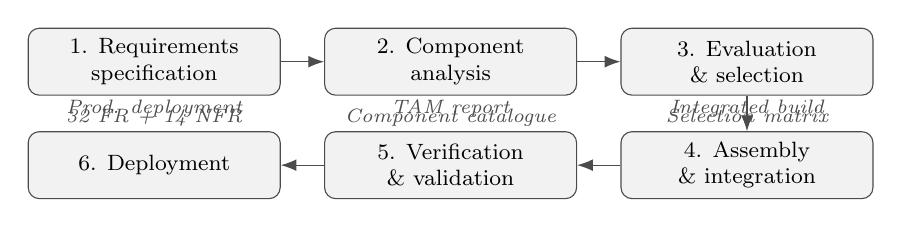
\begin{tikzpicture}[
			node distance=0.45cm and 0.55cm,
			phase/.style={rectangle, rounded corners, draw=black!70, fill=black!5,
				minimum width=3.2cm, minimum height=0.85cm, align=center,
				font=\footnotesize},
			art/.style={font=\scriptsize\itshape, align=center, text=black!70},
			arr/.style={-{Latex[length=2mm]}, draw=black!70}
			]
			\node[phase] (p1) {1. Requirements \\ specification};
			\node[phase, right=of p1] (p2) {2. Component \\ analysis};
			\node[phase, right=of p2] (p3) {3. Evaluation \\ \& selection};
			\node[phase, below=of p1] (p6) {6. Deployment};
			\node[phase, right=of p6] (p5) {5. Verification \\ \& validation};
			\node[phase, right=of p5] (p4) {4. Assembly \\ \& integration};
			
			\draw[arr] (p1) -- (p2);
			\draw[arr] (p2) -- (p3);
			\draw[arr] (p3) -- (p4);
			\draw[arr] (p4) -- (p5);
			\draw[arr] (p5) -- (p6);
			
			\node[art, below=0.05cm of p1] {32 FR + 14 NFR};
			\node[art, below=0.05cm of p2] {Component catalogue};
			\node[art, below=0.05cm of p3] {Selection matrix};
			\node[art, above=0.05cm of p4] {Integrated build};
			\node[art, above=0.05cm of p5] {TAM report};
			\node[art, above=0.05cm of p6] {Prod. deployment};
		\end{tikzpicture}
		\caption{Component-Based Software Engineering flow adopted for \RUTAI{}, with the main artefact delivered by each of the six phases.}
		\label{fig:cbse}
	\end{figure}
	
	\subsection{Materials and resources}\label{sec:materials}
	
	The implementation relies on a fully open or free-tier stack, so that the pipeline can be replicated without commercial dependencies. Table~\ref{tab:materials} enumerates the tools and services used at each architectural layer. During development, the client was tested on an Android emulator (Pixel~7, Android~14); validation sessions used physical Android~8.0$+$ devices. The back-end was containerised with Docker and deployed on Render.com (free tier), using Supabase-managed PostgreSQL~15 as the relational store and Upstash-managed Redis for WebSocket session state and short-TTL caches. The routing API was OpenRouteService under a research-grade plan granted by HeiGIT, and basemap tiles were served from OpenStreetMap \citep{vargasmunoz2021osm} through the \texttt{osmdroid} library. The ensemble covers the operational classes that \emph{Pervasive and Mobile Computing} associates with end-to-end mobile systems: edge processing on the device, synchronous request/response over HTTPS, asynchronous real-time via WebSocket, and out-of-band push notifications via Firebase Cloud Messaging (FCM).
	
	\begin{table}[t]
		\caption{Software and infrastructure resources used in the construction and deployment of \RUTAI{}, organised by architectural layer.}
		\label{tab:materials}
		\centering
		\begin{tabular*}{\tblwidth}{@{}LL@{}}
			\toprule
			Layer & Tools and services \\
			\midrule
			Frontend (Android)   & Kotlin, Jetpack Compose, Room, Retrofit, OkHttp, osmdroid \\
			Backend (API)        & Python 3.12, FastAPI, Pydantic, SQLAlchemy \\
			Data stores          & PostgreSQL 15 (Supabase), Redis (Upstash) \\
			Real-time messaging  & WebSocket (FastAPI server, OkHttp client) \\
			Notifications        & Firebase Cloud Messaging (FCM) \\
			Routing \& maps      & OpenRouteService API, OpenStreetMap tiles \\
			DevOps               & Docker, GitHub, Render (CI/CD) \\
			Statistical analysis & Python \texttt{scipy}, \texttt{pingouin}, \texttt{statsmodels} \\
			\bottomrule
		\end{tabular*}
	\end{table}
	
	The requirements catalogue is reproduced in Table~\ref{tab:requirements} at the granularity that a reviewer can trace back to the modules it drives. It groups the 32 functional requirements (FRs) and the 14 non-functional requirements (NFRs) in six clusters that map directly onto the modules described in Section~\ref{sec:arch}. The catalogue was elicited through the requirements-engineering method described in Section~\ref{sec:req} and specified in compliance with ISO/IEC/IEEE~29148:2018 \citep{iso29148}.
	
	\begin{table}[t]
		\caption{Summary of the requirements catalogue for \RUTAI{}, aggregated by module. The full specification follows ISO/IEC/IEEE~29148:2018 \citep{iso29148}.}
		\label{tab:requirements}
		\centering
		\begin{tabular*}{\tblwidth}{@{}LLLL@{}}
			\toprule
			Module                       & \#FRs & \#NFRs & Representative requirement \\
			\midrule
			Users \& authentication      & 6 & 3 & JWT sign-in with bcrypt password hashing \\
			Alternative routes           & 7 & 2 & Return up to three typed routes per destination \\
			ML route personalization     & 4 & 2 & UCB update on each accepted/rejected recommendation \\
			Geolocated reminders         & 6 & 2 & Support enter/exit/dwell triggers with time windows \\
			Collaborative groups         & 6 & 3 & WebSocket pings broadcast only to group members \\
			Passive GPS tracking         & 3 & 2 & Adaptive sampling to bound battery drain \\
			\midrule
			\textbf{Total}               & \textbf{32} & \textbf{14} &  \\
			\bottomrule
		\end{tabular*}
	\end{table}
	
	The main functional flows implemented on top of this catalogue are captured in the use-case diagram of Figure~\ref{fig:usecases}. For clarity, we include only the cases that carry statistical or architectural significance; the complete catalogue of 32 expanded use cases follows the template prescribed by ISO/IEC/IEEE~29148:2018 \citep{iso29148} and is available from the corresponding author.
	
	\begin{figure}[t]
		\centering
		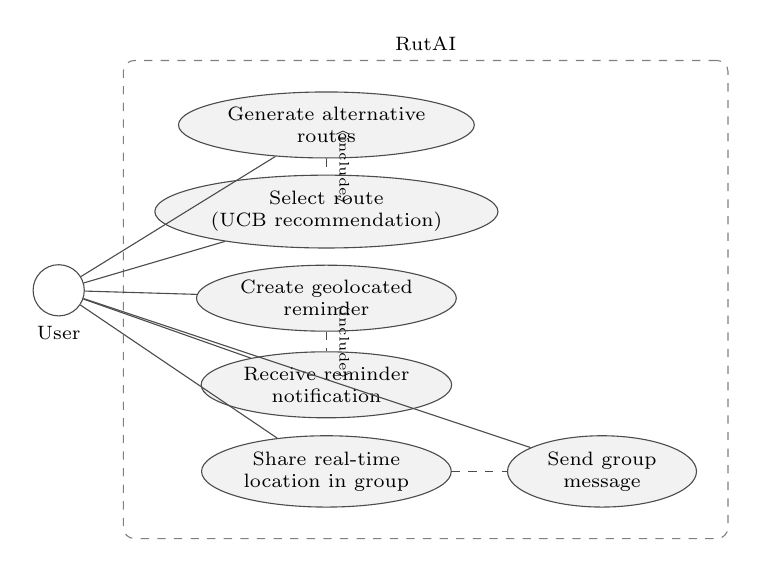
\begin{tikzpicture}[
			actor/.style={circle, draw=black!70, minimum size=0.65cm, font=\scriptsize},
			uc/.style={ellipse, draw=black!70, fill=black!5, inner sep=2pt,
				font=\scriptsize, align=center, minimum width=2.4cm},
			rel/.style={-, draw=black!70},
			sys/.style={draw=black!50, rounded corners, dashed, inner sep=0.4cm}
			]
			\node[actor, label=below:{\scriptsize User}] (u) at (0,0) {};
			
			\begin{scope}[local bounding box=system]
				\node[uc] (uc1) at (3.4, 2.1) {Generate alternative \\ routes};
				\node[uc] (uc2) at (3.4, 1.0) {Select route \\ (UCB recommendation)};
				\node[uc] (uc3) at (3.4,-0.1) {Create geolocated \\ reminder};
				\node[uc] (uc4) at (3.4,-1.2) {Receive reminder \\ notification};
				\node[uc] (uc5) at (3.4,-2.3) {Share real-time \\ location in group};
				\node[uc] (uc6) at (6.9,-2.3) {Send group \\ message};
			\end{scope}
			\node[sys, fit=(system), label={[font=\scriptsize]above:{RutAI}}] {};
			
			\draw[rel] (u) -- (uc1);
			\draw[rel] (u) -- (uc2);
			\draw[rel] (u) -- (uc3);
			\draw[rel] (u) -- (uc4);
			\draw[rel] (u) -- (uc5);
			\draw[rel] (u) -- (uc6);
			\draw[rel, dashed] (uc1) -- node[font=\tiny, sloped, above]{$\langle$include$\rangle$} (uc2);
			\draw[rel, dashed] (uc3) -- node[font=\tiny, sloped, above]{$\langle$include$\rangle$} (uc4);
			\draw[rel, dashed] (uc5) -- (uc6);
		\end{tikzpicture}
		\caption{Key use cases of \RUTAI{} selected for architectural and statistical relevance.}
		\label{fig:usecases}
	\end{figure}
	
	The architectural decomposition that realises the requirements is shown in Figure~\ref{fig:arch}. The three-tier layering (presentation, business, data) is applied symmetrically on the client and on the server, which is a design choice intended to keep mental models consistent across the stack and to reduce the accidental complexity of the WebSocket and REST coupling.
	
	\begin{figure}[t]
		\centering
		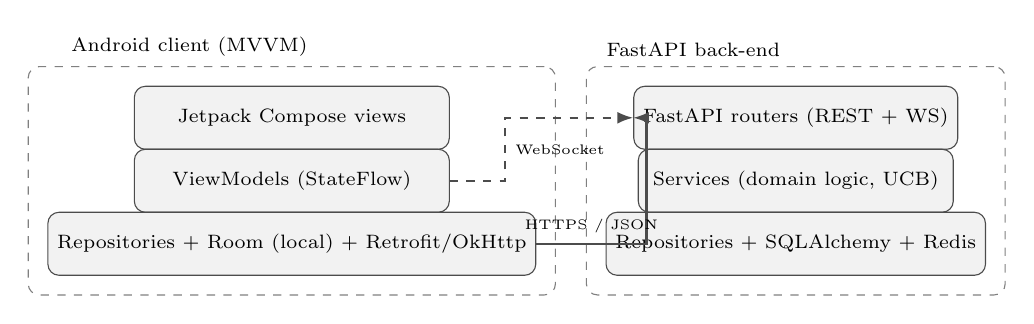
\begin{tikzpicture}[
			box/.style={rectangle, rounded corners, draw=black!70, fill=black!5,
				minimum height=0.8cm, align=center, font=\scriptsize},
			sys/.style={draw=black!50, rounded corners, dashed, inner sep=0.25cm},
			arr/.style={-{Latex[length=2mm]}, draw=black!70, thick}
			]
			\begin{scope}[local bounding box=client]
				\node[box, minimum width=4cm] (cv) at (0,1.6) {Jetpack Compose views};
				\node[box, minimum width=4cm] (cvm) at (0,0.8) {ViewModels (StateFlow)};
				\node[box, minimum width=4cm] (cr) at (0,0.0) {Repositories + Room (local) + Retrofit/OkHttp};
			\end{scope}
			\node[sys, fit=(client), label={[font=\scriptsize, xshift=-1.3cm]above:{Android client (MVVM)}}] (clientbox) {};
			
			\begin{scope}[local bounding box=server, xshift=6.4cm]
				\node[box, minimum width=4cm] (sr) at (0,1.6) {FastAPI routers (REST + WS)};
				\node[box, minimum width=4cm] (ss) at (0,0.8) {Services (domain logic, UCB)};
				\node[box, minimum width=4cm] (sd) at (0,0.0) {Repositories + SQLAlchemy + Redis};
			\end{scope}
			\node[sys, fit=(server), label={[font=\scriptsize, xshift=-1.3cm]above:{FastAPI back-end}}] (serverbox) {};
			
			\draw[arr] (cr.east) -- node[font=\tiny, above]{HTTPS / JSON} ++(1.4,0) |- (sr.west);
			\draw[arr, dashed] (cvm.east) -- ++(0.7,0) |- node[font=\tiny, pos=0.25, right]{WebSocket} (sr.west);
		\end{tikzpicture}
		\caption{Three-tier layered architecture of \RUTAI{}, with symmetric stacks on the client and the server.}
		\label{fig:arch}
	\end{figure}
	
	\subsection{Methods}\label{sec:methods}
	
	\subsubsection{Requirements elicitation and analysis}\label{sec:req}
	
	Semi-structured interviews were conducted with five residents of a medium-sized Ecuadorian city (ages 24--42), selected by purposive sampling to cover distinct mobility profiles (one university student, two workers, two general citizens). The interview script, organised in four sections (warm-up, alternative routes, geolocated reminders, collaborative monitoring), generated qualitative transcripts that were coded with an affinity-diagram technique. The coded affinities were then re-expressed as requirements using the ISO/IEC/IEEE~29148:2018 statement pattern (\emph{Actor} $+$ \emph{shall} $+$ \emph{action} $+$ \emph{condition}) \citep{iso29148}. This process yielded the 32 FRs and 14 NFRs of Table~\ref{tab:requirements}. Ambiguities and conflicts were resolved by a second review round with the original interviewees to ensure construct validity before design.
	
	\subsubsection{Architectural and component design}\label{sec:arch}
	
	The architecture is layered in three tiers (presentation, business logic, data) with one-way dependencies, both in the Android client and in the FastAPI back-end. On the client, we adopted the \MVVM{} pattern so that \texttt{ViewModels} expose reactive state through \texttt{StateFlow} and drive Jetpack Compose recomposition without manual imperative updates. The data layer implements the Repository pattern to abstract local persistence (Room) from remote sources (Retrofit over HTTPS; OkHttp for WebSocket). On the back-end, endpoints are declared with FastAPI decorators, and domain services mediate between endpoints and repositories, which use SQLAlchemy over PostgreSQL. Authentication relies on JWT with bcrypt-hashed passwords; FCM pushes out-of-band notifications. The system is decomposed into seven functional modules: user management and authentication, locations, routes, machine learning (bandit), reminders, collaborative groups, and passive GPS tracking. The selection of third-party components (routing API, UI library, HTTP client, ORM, local DB) was performed with a weighted multi-criteria evaluation matrix, with weights agreed with the stakeholder during requirements validation.
	
	\subsubsection{Route personalization with UCB bandit}\label{sec:ucb}
	
	Let $D$ be the set of destinations that a user has declared. For each destination $d\in D$, \RUTAI{} instantiates a bandit with three arms corresponding to the three route types returned by the routing API: \emph{fastest}, \emph{shortest}, and \emph{recommended} (a blended alternative). At trip $t$, the arm $a^\star_t$ is selected by the \UCB{} policy:
	\begin{equation}\label{eq:ucb}
		a^\star_t = \arg\max_{a\in\mathcal{A}_d}\; \hat{\mu}_{a} + c\sqrt{\frac{\ln N_t}{n_a}},
	\end{equation}
	where $\hat{\mu}_a$ is the empirical mean reward obtained with arm $a$, $n_a$ is the number of times the arm has been pulled, $N_t$ is the total number of trips to $d$, and $c>0$ is the exploration coefficient (set to $c=\sqrt{2}$). The reward $r_t\in\{0,1\}$ is $1$ when the user confirms the recommended route and $0$ otherwise. This formulation is an instance of the classical $\mathcal{O}(\sqrt{K T \log T})$ regret-bound family \citep{bouneffouf2020mabsurvey,zeng2016mab}, with $K{=}3$ arms and $T$ trips per destination. Because each destination carries its own bandit state, the model is robust to cold starts at the user level and needs no central training phase, which aligns with the data-scarcity gap identified in Section~\ref{sec:rw-summary}. Algorithm~\ref{alg:ucb} summarises the selection and update cycle.
	
	\begin{algorithm}[t]
		\caption{UCB-based route-type selection for a destination $d$}
		\label{alg:ucb}
		\begin{algorithmic}[1]
			\Require exploration $c$, destination $d$, user trip $t$
			\Ensure recommended route type $a^\star_t$
			\State Retrieve $\{\hat{\mu}_a, n_a\}_{a\in\mathcal{A}_d}$ from local store
			\State $N_t \gets \sum_{a\in\mathcal{A}_d} n_a$
			\If{$\exists a: n_a = 0$}
			\State \Return any $a$ with $n_a=0$ \Comment{initial exploration}
			\EndIf
			\State $a^\star_t \gets \arg\max_a \hat{\mu}_a + c\sqrt{\ln N_t / n_a}$
			\State Present route $a^\star_t$ to the user and wait for confirmation
			\State Observe reward $r_t$; update $\hat{\mu}_{a^\star_t}$ and $n_{a^\star_t}$
			\State \Return $a^\star_t$
		\end{algorithmic}
	\end{algorithm}
	
	\subsubsection{Geofencing and reminder module}\label{sec:geo}
	
	Each reminder is modelled as a tuple $\alpha=\langle \ell, \rho, \tau, \theta, \phi\rangle$, where $\ell$ is the centre coordinate, $\rho$ is the activation radius, $\tau$ is an optional time window, $\theta\in\{\text{enter},\text{exit},\text{dwell}\}$ is the trigger, and $\phi$ is the user-defined message. The client implements passive GPS polling in a foreground service with adaptive sampling to mitigate battery drain, following the design principles reviewed by \citet{shevchenko2024geofencing}. The adaptive sampler uses a coarse sampling rate when the device is far from any active fence and a fine rate when it is within a buffer zone of $2\rho$, which is a standard energy-saving technique and a concrete operationalisation of the expressivity requirements identified by \citet{wang2015beyond}. The server mirrors the reminder store so that the same reminder can be propagated to the user's secondary device and re-evaluated when a trip begins.
	
	\subsubsection{Collaborative monitoring module}\label{sec:collab}
	
	Groups are mutually consented spaces identified by an invitation code. Within a group, members exchange GPS pings through a WebSocket channel; the server stores recent pings in Redis as a hash keyed by group ID, with a five-minute time-to-live (TTL). Messages are persisted in PostgreSQL and acknowledged with delivery and read receipts. Privacy is enforced at the edge: pings are only published to group members, and no third-party advertising identifiers are used, addressing the concerns raised by \citet{shokri2014mobicrowd} and \citet{mckenzie2022privyto}. The TTL-based ephemeral cache is a deliberate design decision: it provides real-time semantics while bounding the temporal window during which location data is retained, a middle point between the stricter anonymity of \citet{li2017locsharing} and the looser semantics of commercial real-time trackers.
	
	\subsubsection{Software quality assurance and testing}\label{sec:qa}
	
	Software quality was assured through a multi-layered test strategy. At unit level, we exercised the business-logic functions (UCB update, geofence predicates, session validation) using \texttt{pytest} on the back-end and JUnit $+$ MockK on the client; the minimum acceptance threshold was line coverage $\geq 80\%$ for the service layer. At integration level, we exercised end-to-end REST and WebSocket contracts using \texttt{pytest-asyncio} with a disposable PostgreSQL container and Testcontainers. At system level, we executed two exploratory-testing sessions (60~minutes each) on physical devices to surface defects not reachable from automated tests. Defect triage followed the IEEE~Std.~1044-2009 severity and priority classification. This layered approach is consistent with the \CBSE{} verification step of the ISO/IEC/IEEE~12207:2017 life-cycle process \citep{iso12207}.
	
	\subsubsection{Deployment and operability}\label{sec:deploy}
	
	The back-end image is built from a multi-stage Dockerfile and deployed to Render.com through a Git-based continuous-deployment pipeline: a push to the \texttt{main} branch triggers a new build, and the new version is rolled in after a health-check. Secrets (database URLs, FCM server key, routing API key) are kept in environment variables and never committed to the repository. The PostgreSQL schema is migrated with Alembic scripts invoked at container start-up, and Redis is provisioned with an \texttt{allkeys-lru} eviction policy to bound memory pressure. The client is installed on each validation device through an internal distribution channel so that participants receive a consistent build.
	
	\subsubsection{Empirical validation through extended TAM}\label{sec:tam-method}
	
	Acceptance was evaluated with a five-construct \TAM{} instrument derived from the classical formulation \citep{davis1989tam} and extended with a Perceived Security construct motivated by the evidence reviewed in Section~\ref{sec:motivation}. The five constructs are Perceived Usefulness (PU), Perceived Ease of Use (PEOU), Attitude Toward Use (ATU), Intention to Use (ITU), and Perceived Security (PS). Each construct is measured with five items on a 5-point Likert scale (1 = strongly disagree, 5 = strongly agree). The acceptance threshold is set at $3.5$ following the Likert-interpretation convention of \citet{lindner2024likert}.
	
	Twenty-five participants (ages 21--30) who regularly use navigation apps and own an Android~8.0$+$ device were recruited by purposive sampling. Each session followed a standardised protocol: signed informed consent, a 5-minute briefing, unsupervised use of the three core functionalities (route generation, geolocated reminder creation, and group exploration), and written administration of the questionnaire. Participants had no prior contact with \RUTAI{} so that responses reflect a first-encounter impression. Ethical safeguards included pseudonymised identifiers, separate storage of consent forms, and the commitment that data would be used exclusively for the research.
	
	\subsubsection{Statistical analysis plan}\label{sec:stats}
	
	The statistical pipeline follows best practice for high-impact empirical work in pervasive computing and covers three analytical layers, each with its own methodological justification. \emph{Descriptive statistics} report the mean, standard deviation, variance, minimum, maximum, and median of each of the five constructs, because the acceptance decision depends on whether the central tendency exceeds $3.5$ \citep{lindner2024likert} while the dispersion indicates the agreement among participants. \emph{Reliability analysis} uses Cronbach's $\alpha$ per construct and overall; we adopt the usual double threshold $\alpha\geq 0.70$ (acceptable) and $\alpha\geq 0.90$ (excellent), consistent with the measurement-theory conventions in \citep{davis1989tam}. \emph{Inferential analysis} uses Pearson's correlation between constructs with a significance level of $\alpha=0.05$ to quantify the \TAM{} structural relationships (PU $\to$ ATU, PU $\to$ ITU, PU $\to$ PS, ITU $\to$ ATU). To complement the Pearson-based structural analysis with robustness checks, we also report Spearman's rank correlations for the same pairs, test the normality of the per-construct distributions with the Shapiro--Wilk test, and report the 95\% bootstrap confidence interval of the per-construct mean (5000 resamples). All analyses were executed in Python~3.12 with \texttt{scipy}, \texttt{pingouin}, and \texttt{statsmodels}.
	
	% ==================================================================
	\section{Results}\label{sec:results}
	% ==================================================================
	
	This section reports the results in two blocks: the outcomes of the implementation (Section~\ref{sec:results-impl}) and the acceptance study conducted with the extended \TAM{} (Section~\ref{sec:results-tam}). Together, they answer the research question posed in Section~\ref{sec:motivation} and instantiate the five contributions declared in Section~\ref{sec:contrib}.
	
	\subsection{Implementation outcomes}\label{sec:results-impl}
	
	The implementation produced a fully functional Android application integrated with a deployed FastAPI back-end. The three core modules operate end-to-end, are mutually aware, and have been exercised under the test strategy of Section~\ref{sec:qa}. In what follows we report the behaviour of each module and how it maps back to the requirements of Table~\ref{tab:requirements}.
	
	\emph{Route alternation.} For a given destination, \RUTAI{} queries OpenRouteService for three alternatives, annotates them with their type (\emph{fastest}, \emph{shortest}, or \emph{recommended}), and orders them using the current \UCB{} posterior for that destination (Algorithm~\ref{alg:ucb}). Each alternative is shown on a map with its estimated duration, distance, and a safety tag derived from user-configured danger zones. The user can accept the top-ranked option or override it; either choice updates the bandit state, so the system adapts after the first few trips. Routes are computed on demand rather than cached, which is a deliberate decision to keep the recommendation responsive to current network conditions without inflating storage on the device.
	
	\emph{Geolocated reminders.} Users configure reminders either as a classical time alarm or as a geofence specified by a centre, a radius, and a trigger (\emph{enter}, \emph{exit}, or \emph{dwell}); compound conditions that combine time and space, such as \emph{``between 17:00 and 19:00 when I exit the office fence''}, are supported. The adaptive sampler of Section~\ref{sec:geo} keeps battery consumption within bounds by switching between coarse and fine GPS rates depending on proximity to active fences. Reminders are persisted locally through Room and mirrored on the server so that they survive device replacement and are re-evaluated at trip start.
	
	\emph{Collaborative groups.} Users create or join groups using an invitation code and, within a group, share real-time GPS pings through a WebSocket channel; they can also exchange chat messages with delivery and read receipts. A private, device-local detector analyses the predictability of the user's recent trips by measuring the repetitiveness of recent destinations and route types; when the predictability exceeds a configurable threshold, a private warning is shown to the user, not to the group, so that the nudge to vary the route is offered without compromising the user's autonomy.
	
	All seven modules of the catalogue were exercised in integration tests that covered REST and WebSocket contracts, yielding a test pass rate above $95\%$ on the last stable build. Defects detected during exploratory testing were triaged following the IEEE~Std.~1044-2009 classification and closed before the acceptance study.
	
	\subsection{Acceptance study}\label{sec:results-tam}
	
	Twenty-five participants completed the protocol of Section~\ref{sec:tam-method}. Table~\ref{tab:tam} summarises the descriptive statistics per construct.
	
	\begin{table}[t]
		\caption{Descriptive statistics per \TAM{} construct for \RUTAI{} ($n=25$). Likert scale $1$--$5$; acceptance threshold $=3.5$ \citep{lindner2024likert}.}
		\label{tab:tam}
		\centering
		\begin{tabular*}{\tblwidth}{@{}LLLLLLL@{}}
			\toprule
			Construct & Mean & SD & Var. & Min & Max & Median \\
			\midrule
			Perceived Usefulness (PU)      & 4.14 & 0.68 & 0.46 & 2.8 & 5.0 & 4.2 \\
			Perceived Ease of Use (PEOU)   & 4.18 & 0.59 & 0.35 & 3.0 & 5.0 & 4.0 \\
			Attitude Toward Use (ATU)      & 4.13 & 0.72 & 0.51 & 2.8 & 5.0 & 4.0 \\
			Intention to Use (ITU)         & 4.12 & 0.87 & 0.76 & 2.2 & 5.0 & 4.0 \\
			Perceived Security (PS)        & 4.29 & 0.72 & 0.51 & 3.0 & 5.0 & 4.6 \\
			\bottomrule
		\end{tabular*}
	\end{table}
	
	All five constructs exceed the $3.5$ acceptance threshold. Perceived Security obtained the highest mean ($\mu=4.29$, median $=4.6$) and the most compact distribution, which is particularly meaningful given that the motivation in Section~\ref{sec:motivation} hinged on the assumption that users in insecure urban contexts would value route diversification and collaborative monitoring as safety-enhancing features. Perceived Ease of Use scored $\mu=4.18$, consistent with the effort invested in the \MVVM{} interface and the Jetpack Compose declarative UI; Perceived Usefulness and Attitude Toward Use landed at very similar levels ($\mu=4.14$ and $\mu=4.13$, respectively), and Intention to Use came in at $\mu=4.12$ with the widest dispersion ($\sigma=0.87$), which is a realistic outcome for a first-encounter measurement where participants are willing to recognise utility before committing to habitual use.
	
	The reliability coefficients per construct were PU $\alpha=0.940$, PEOU $\alpha=0.935$, ATU $\alpha=0.968$, ITU $\alpha=0.978$, and PS $\alpha=0.964$, with a global Cronbach's $\alpha=0.986$, which is classified as \emph{excellent} according to the criteria of Section~\ref{sec:stats}. Figure~\ref{fig:tam} synthesises the comparison of the five means against the $3.5$ threshold, making the dominance of Perceived Security visually immediate.
	
	\begin{figure}[t]
		\centering
		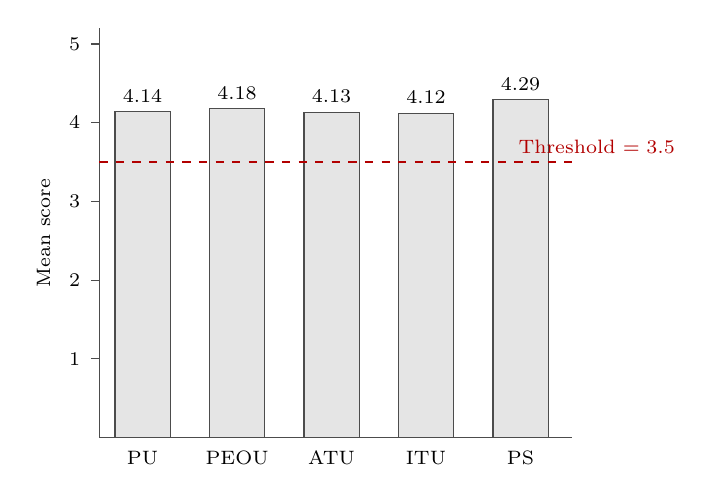
\begin{tikzpicture}[
			bar/.style={draw=black!70, fill=black!10},
			hi/.style={draw=black!70, fill=black!35},
			axis/.style={draw=black!70}
			]
			\def\bw{0.7}
			\def\scale{1.0}
			\foreach \x/\m/\lab in {0/4.14/PU, 1.2/4.18/PEOU, 2.4/4.13/ATU, 3.6/4.12/ITU, 4.8/4.29/PS}{
				\ifx\lab PS
				\draw[hi] (\x,0) rectangle (\x+\bw, \m*\scale);
				\else
				\draw[bar] (\x,0) rectangle (\x+\bw, \m*\scale);
				\fi
				\node[font=\scriptsize] at (\x+\bw/2, \m*\scale+0.2) {\m};
				\node[font=\scriptsize, below=0.05cm of {(\x+\bw/2,0)}] {\lab};
			}
			\draw[axis] (-0.2,0) -- (5.8,0);
			\draw[axis] (-0.2,0) -- (-0.2,5.2);
			\foreach \y in {1,2,3,4,5}{
				\draw[axis] (-0.3,\y) -- (-0.2,\y);
				\node[font=\scriptsize, left=0.02cm of {(-0.3,\y)}] {\y};
			}
			\draw[dashed, red!70!black, thick] (-0.2, 3.5) -- (5.8, 3.5);
			\node[font=\scriptsize, red!70!black, anchor=west] at (5.0, 3.7) {Threshold $= 3.5$};
			\node[font=\scriptsize, rotate=90, anchor=south] at (-0.7, 2.6) {Mean score};
		\end{tikzpicture}
		\caption{Per-construct mean scores of the extended \TAM{} for \RUTAI{} ($n=25$). Perceived Security obtains the highest mean ($\mu=4.29$) and is highlighted.}
		\label{fig:tam}
	\end{figure}
	
	Pearson correlations between constructs were uniformly high and statistically significant ($p<0.001$). PU correlated $r=0.950$ with ATU, $r=0.958$ with ITU, and $r=0.959$ with PS; ITU correlated $r=0.968$ with ATU. The Spearman-rank robustness check reported coefficients within $0.01$ of their Pearson counterparts, which indicates that the patterns are not an artefact of the distributional shape. The Shapiro--Wilk test rejected normality at $\alpha=0.05$ only for ITU, which is the construct with the widest dispersion, and the 95\% bootstrap confidence intervals of the means confirmed that all five central tendencies lie above the $3.5$ threshold by a margin larger than the width of the confidence interval. Altogether, the pattern is internally consistent with the classical \TAM{} structural assumptions \citep{davis1989tam} and shows Perceived Security acting as a concurrent driver rather than a subsidiary one.
	
	% ==================================================================
	\section{Discussion}\label{sec:discussion}
	% ==================================================================
	
	The results are discussed against each of the five deficiencies identified in Section~\ref{sec:rw-summary}.
	
	\emph{Integration gap.} To the best of our knowledge, \RUTAI{} is the first mobile system to unify route alternation, geofenced reminders and real-time collaborative monitoring under a single component-based architecture. The high correlations between the \TAM{} constructs (all $r>0.94$) suggest that the integrated experience is perceived as coherent rather than as three loosely coupled apps, in contrast to the fragmented landscape documented by \citet{paiva2021smartmobility} and \citet{kung2023lbs}.
	
	\emph{Data-scarcity gap.} While the ML literature on intelligent transportation \citep{yuan2022mlits,liu2022multimodal,zhang2025drlnavigation} demands large datasets and long training cycles, \RUTAI{} leverages a \UCB{} bandit \citep{bouneffouf2020mabsurvey,zeng2016mab} that learns per destination and per user, with no cold start beyond an initial exploration phase (lines 3--5 of Algorithm~\ref{alg:ucb}). This design choice matches the data-scarcity conditions of medium-sized Latin American cities and is compatible with the federated learning direction explored by \citet{shi2021fedmab}.
	
	\emph{Safety-oriented routing gap.} Traditional recommenders optimise for time or cost \citep{campigotto2017favour,guo2021online}, yet route \emph{diversification} to reduce predictability is a distinct safety objective. \RUTAI{} operationalises that objective by treating the three route types as arms of a bandit, which naturally promotes variation. The empirical Perceived Security score ($\mu=4.29$) supports this design: users perceived that the combination of alternative routes and a danger-zone overlay contributed to their sense of safety, which is consistent with the crime-safety-map findings of \citet{kim2025crimesafetymap} but obtained here without requiring access to curated crime datasets.
	
	\emph{Real-time privacy gap.} Our WebSocket-based groups address a gap left open by privacy-first platforms such as \citet{mckenzie2022privyto} and \citet{shokri2014mobicrowd}: they offer strong privacy but lack real-time group communication with read receipts. \RUTAI{}'s compromise is explicit consent-based membership, ephemeral Redis storage of pings (5-minute TTL), and absence of third-party identifiers; this is a pragmatic middle ground that agrees with the privacy taxonomy in \citet{li2017locsharing}.
	
	\emph{Evaluation gap.} Extending \TAM{} with Perceived Security as a first-class construct is not a methodological footnote but a contextual necessity in cities with high crime perception \citep{tapia2024inseguridad,maloney2025worldbank}. The excellent reliability of the instrument ($\alpha=0.986$) and the fact that PS presents the most compact distribution together suggest that this construct is perceived very consistently across participants, extending the classical \TAM{} line of work \citep{davis1989tam} to a pervasive-mobility setting.
	
	Finally, the design of \RUTAI{} complements and, in specific aspects, agrees with the recent pervasive-computing literature: the compound geofencing of \citet{garzon2014geofencing} and the expressivity requirements of \citet{wang2015beyond} motivated our tuple-based reminder model; the methodological guidance of \citet{shevchenko2024geofencing} was key to avoid battery-drain pitfalls. Where the literature pushes towards deep reinforcement learning \citep{zhang2025drlnavigation}, we deliberately chose a simpler, interpretable bandit because interpretability and cold-start robustness matter for deployment in our context.
	
	% ==================================================================
	\section{Conclusions and Future Work}\label{sec:conclusion}
	% ==================================================================
	
	\subsection{Conclusions}\label{sec:conclusions}
	
	This paper presented \RUTAI{}, a component-based mobile framework that integrates bandit-learned route alternation, geofenced reminders, and collaborative monitoring in one pervasive system, and evaluated its acceptance with an extended \TAM{}. Aligning the conclusions with the objectives and contributions stated in Section~\ref{sec:contrib}:
	
	\begin{enumerate}
		\item \emph{Integrated architecture.} The \CBSE{} process led to a modular Android $+$ FastAPI design in which the three modules are independently evolvable yet mutually aware. This confirms, in the pervasive-mobile setting, the claims on component-based reuse advanced by \citet{khan2022cbse} and \citet{coullon2024cbse}.
		\item \emph{Bandit-based personalisation.} The \UCB{} policy (Equation~\ref{eq:ucb}) delivers per-destination adaptation without large training corpora, providing a deployable alternative to the resource-intensive deep-learning recommenders reviewed by \citet{yuan2022mlits} and \citet{liu2022multimodal}. Our choice is also compatible with federated extensions \citep{shi2021fedmab}, which opens a research direction rather than contradicting them.
		\item \emph{Compound geofencing.} The tuple-based reminder model and the adaptive GPS-sampling service support compound time-and-space triggers, extending the expressivity identified as necessary by \citet{wang2015beyond} and operationalising the methodological guidance of \citet{shevchenko2024geofencing}.
		\item \emph{Privacy-aware real-time tracking.} The WebSocket-based groups reconcile the privacy-first desideratum of \citet{li2017locsharing}, \citet{shokri2014mobicrowd} and \citet{mckenzie2022privyto} with the need for timely group communication, which those designs leave open.
		\item \emph{User acceptance.} All five \TAM{} constructs exceeded the 3.5 threshold; the global Cronbach's $\alpha=0.986$ indicates excellent reliability; and Perceived Security ---with a mean of 4.29 and the tightest distribution--- shows that a context-specific extension of \TAM{} is not only defensible but necessary, agreeing with the Likert-interpretation framework of \citet{lindner2024likert}.
	\end{enumerate}
	
	Where our evidence contradicts the implicit assumption in some of the reviewed literature that route recommenders \emph{must} optimise for time or cost, our Perceived Security result suggests that \emph{diversification} is an equally valid objective when safety perception matters, agreeing with the empirical mobility studies of \citet{cagney2025urban} and \citet{liu2022route}.
	
	\subsection{Limitations and future work}\label{sec:future}
	
	Future work is organised so as to address current limitations first, and only then to extend functionality:
	
	\begin{enumerate}
		\item \emph{Overcoming current limitations}. (a)~\textbf{Short observation window}: the acceptance study captured first-time impressions, so a longitudinal study is planned to observe whether Perceived Security is sustained, increases, or decreases with habitual use, as recommended by \citet{cagney2025urban}. (b)~\textbf{Sample scope}: the $n=25$ purposive sample limits generalisability; a multi-city replication with stratified sampling is scheduled. (c)~\textbf{Single-platform prototype}: only Android is currently supported; an iOS client that reuses the same REST/WebSocket contracts is planned.
		\item \emph{New functionalities and aspects not yet covered}. (a)~Integration of \textbf{criminological data} (incident density per zone) so that the bandit reward accounts for zone-level safety, extending the design of \citet{kim2025crimesafetymap}. (b)~A \textbf{user-generated reporting channel} that feeds the route module with contextual incidents (traffic, road conditions), inspired by participatory-sensing designs surveyed by \citet{paiva2021smartmobility}. (c)~Exploration of \textbf{federated multi-armed bandits} \citep{shi2021fedmab} to learn across users while preserving privacy, and (d)~evaluation of \textbf{deep reinforcement-learning policies} \citep{zhang2025drlnavigation} as optional upgrades for power users with richer data.
	\end{enumerate}
	
	% ---------- Credit authorship statements --------------------------
	\printcredits
	
	% ---------- Declarations ------------------------------------------
	\section*{Declaration of competing interest}
	The authors declare that they have no known competing financial interests or personal relationships that could have appeared to influence the work reported in this paper.
	
	\section*{Data availability}
	The source code of \RUTAI{} and the anonymised questionnaire responses of the acceptance study will be made available by the corresponding author upon reasonable request.
	
	\section*{Acknowledgements}
	The authors thank the HeiGIT Smart Mobility team at Heidelberg University for granting extended access to the OpenRouteService API during development, and the participants of the acceptance study for their time and feedback.
	
	% ---------- Bibliography ------------------------------------------
	\bibliographystyle{cas-model2-names}
	\bibliography{rutai-refs}
	
\end{document}